\documentclass{beamer}
\usepackage{graphicx}
\usepackage{tikz}
\usetikzlibrary{shapes,arrows}
\usepackage{tikz}
\usetheme{default}
%\usecolortheme{seahorse}
\usepackage{default}
  \setbeamertemplate{footline}[page number]

\setbeamertemplate{navigation symbols}{}
\setbeamertemplate{frametitle}[default][center]
\setbeamerfont{frametitle}{shape=\scshape}

\usepackage{xcolor}

\usepackage[flushleft]{threeparttable}

{\title{\textsc{Course Introduction}}
\date{}
\author{Trevor Gallen}

\begin{document}
\renewcommand*{\inserttotalframenumber}{\pageref{lastframe}}

\begin{frame}
\titlepage
\end{frame}


\begin{frame}
\frametitle{Introduction}
\begin{itemize}
\item Current Topics in Macro
\bigskip
\item Asynchronous
\bigskip
\item No prerequisites
\bigskip
\item Discussion board first, only e-mail for private issues
\bigskip
\item Warning: some videos are old, and from a course in 2020
\end{itemize}
\end{frame}

\begin{frame}
\frametitle{How you do it}
\begin{itemize}
\item Go to course Brightspace
\bigskip
\item Click on Content
\bigskip
\item Click on Syllabus, read it
\bigskip
\item Click on ``Start here" watch this video
\bigskip
\item Go down to ``Macroeconomic Aggregates" and start the course, progress down by week
\end{itemize}
\end{frame}


\begin{frame}
\frametitle{Grading}
\begin{itemize}
\item Course is organized around the principle of being able to competently speak about macro and public policy
\end{itemize}
\begin{table}
\centering
\begin{tabular}{ll}
\hline\hline
Writing prompts (``homeworks") & 50\%\\
Online discussion &  30\% \\
Multiple-choice midterm exam (timed online) &  10\%\\ 
Multiple-choice final exam  (timed online) &  10\% \\
\hline\hline
\end{tabular}
\end{table}
\end{frame}

\begin{frame}
\frametitle{Writing prompts}
\begin{itemize}
\item Writing prompts are workhorse of the course (50\% of grade)
\bigskip
\item Typically, one per week due Saturday night (Sunday first week)
\bigskip
\item Looking for one to two pages, that for instance:
\begin{itemize}
\item Clearly states a response to the question/prompt
\item Delineates any conceptual theory that's relevant
\item Introduces the evidence of relevant papers
\item Introduces any new data the author brings to the argument
\item Addresses flaws or potential weaknesses in the author's argument
\end{itemize} 
\item Goal is to write a short coherent description of the issue, put forward an argument backed by evidence provided by others, new evidence or analysis you might bring to the fore, but is not entirely one-sided, e.g. recognizes its own weaknesses
\end{itemize}
\end{frame}

\begin{frame}
\frametitle{Writing prompt grading}
\begin{figure}
\centering
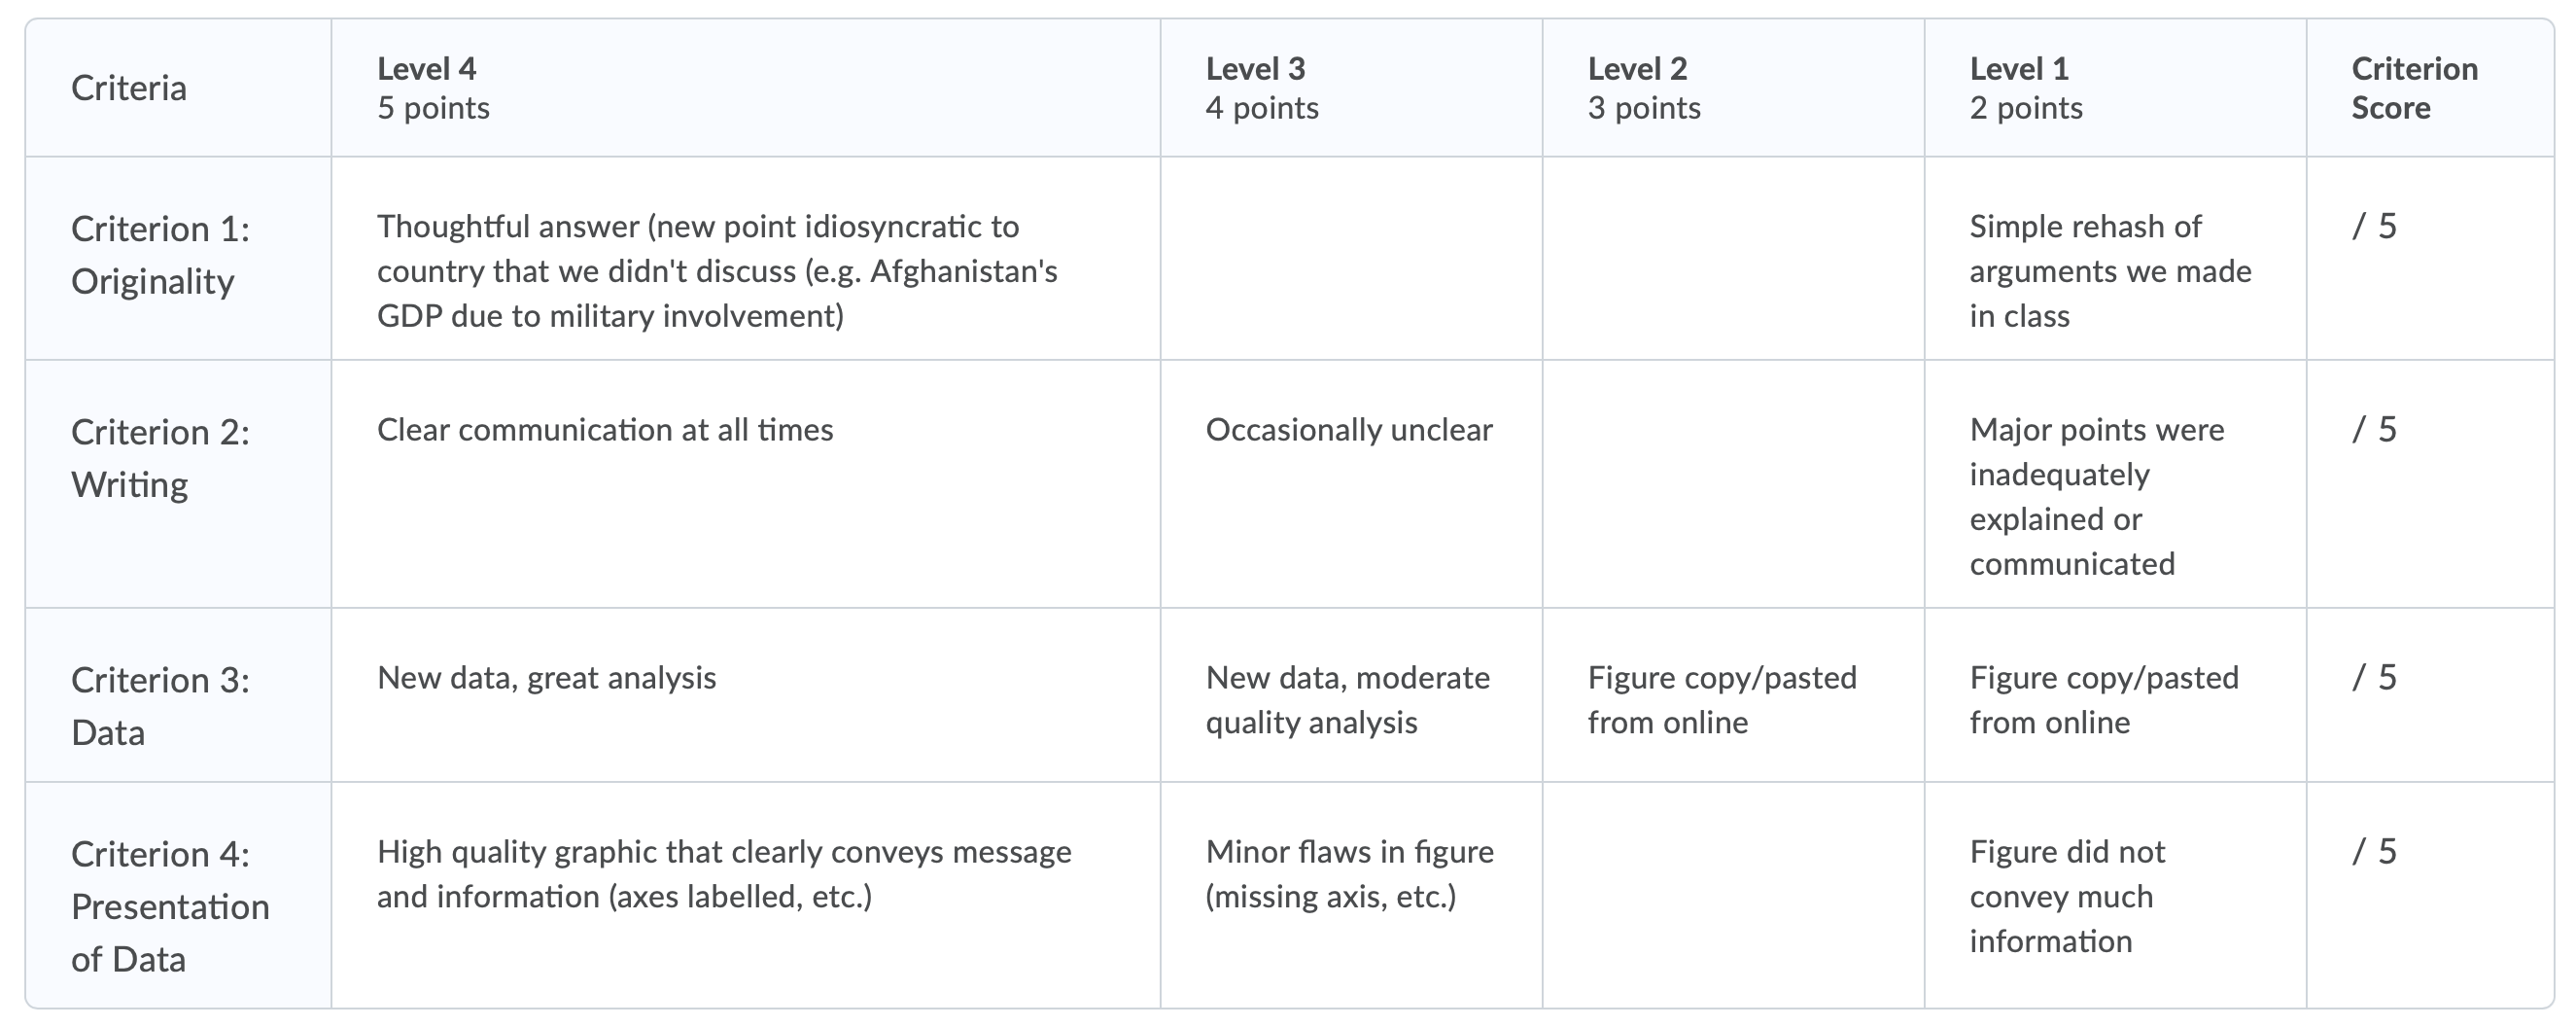
\includegraphics[scale=0.25]{ExampleRubric.png}
\end{figure}
\end{frame}

\begin{frame}
\frametitle{Discussion}
\begin{itemize}
\item Discussion is core to this class (30\%!)
\bigskip
\item Should be civil, but no ideas are out of bounds
\bigskip
\item Best type of discussion (1) takes a position and defends it, (2) questions someone else's position (civilly) (3) attempts to answer someone else's extension or clarifying question
\bigskip
\item Next best asks an extending question (``what about Argentina, which seems to be an exception to the example because XYZ") 
\bigskip
\item Next best is clarifying questions (``is this a typo?" or  ``I didn't understand why we use the Cobb-Douglass production function")
\bigskip
\item Some credit is given for minor course questions
\bigskip
\item Questions that could benefit others should be asked on discussion (public good)
\end{itemize}
\end{frame}

\begin{frame}
\frametitle{Exams}
\begin{itemize}
\item Exams are relatively unimportant (10\% each)
\bigskip
\item Simple multiple choice, possibly a few short response questions
\end{itemize}
\end{frame}

\begin{frame}
\frametitle{Topics}
\begin{itemize}
\item \textbf{Section 1:} Macroeconomic Aggregates (wk 1)
\item \textbf{Section 2:} Labor/Leisure Tradeoff (wk 1)
\item \textbf{Section 3:} Intertemporal Tradeoff (wk 2)
\item \textbf{Section 4:} Crash Course in Growth Theory (wk 2)
\item \textbf{Section 5:} Understanding Immigration (wk 3)
\item \textbf{Section 6:} Robots and Automation (wk 3)
\item \textbf{Section 7:} Inequality (wk 3)
\item \textbf{Section 8:} Social Safety Net and Fiscal Policy (wk 4)
\item \textbf{Section 9:} Universal Basic Income (wk 4)
\item \textbf{Section 10:} Monetary Policy Basics (wk 5)
\item \textbf{Section 11:} Modern Monetary Theory (wk 5)
\item \textbf{Section 12:} Cryptocurrency (wk 5)
\item \textbf{Section 12:} Government Debt (wk 6)
\item \textbf{Section 14:} Bank Runs and US Financial Crisis (wk 7)
\item \textbf{Section 15:} Covid-19 Pandemic (wk 7)
\item \textbf{Section 16:} TBD (wk 8)
\end{itemize}
\end{frame}

\begin{frame}
\frametitle{First chance at discussion}
\begin{itemize}
\item Propose a topic for Week 8 that you feel is missing.  Make the case for it
\bigskip
\item We will vote on it next week
\end{itemize}
\end{frame}

\begin{frame}
\frametitle{OH}
\begin{itemize}
\item I currently have few plans for online OH, spend a long time on discussion boards
\bigskip
\item I may find time for a few, depending on how busy discussion board is!
\end{itemize}
\end{frame}

\end{document}